\section{Terrain following tracer advection}
\label{sec:wobblyTracerAdvection}

In the horizontal advection test, results were more accurate when the flow was aligned with grid layers: on the cut cell grid results were accurate, but distortions in the BTF grid led to increased error.  This terrain following advection test is designed to determine the nature of these errors by prescribing a velocity field that is aligned with the layers of the BTF grid.  If errors are caused by skewness or grid non-uniformity (described in section~\ref{sec:theory:skewness}), we expect least accuracy on terrain following grids since they are less orthogonal.  However, if errors are caused by flow crossing grid layers, then results are expected to be less accurate on the SnapCol grid.

\subsection{Specification}
The spatial domain, mountain profile, initial tracer profile and discretisation are the same as those in the horizontal tracer advection test (section~\ref{sec:advection}).  The velocity field, however, is defined using a streamfunction $\Psi$ so that the velocity field is non-divergent.  Unlike the horizontal advection test, flow extends from the top of the domain all the way to the ground.  It is defined so that flow is everywhere tangential to BTF coordinate surfaces given by equation~\ref{eqn:theory:btf} such that
\begin{align}
	\Psi(x,z) &= H \frac{z - h}{H - h}
%
	\intertext{The horizontal and vertical components of velocity, $u$ and $w$ are then given by}
%
	u &= \frac{\partial \Psi}{\partial z} \quad,\quad  w = -\frac{\partial \Psi}{\partial x}
%
	\intertext{Hence, for the mountain profile given in equation~\ref{eqn:advection:schaerCos} we find}
%
	u &= \frac{H}{H - h} \quad,\quad w = H \frac{\partial h}{\partial x} \frac{H - z}{\left( H - h \right)^2} \label{eqn:wobblyTracerAdvection:velocity} \\
	\frac{\partial h}{\partial x} &= - h_0 \pi \left[ 
		\frac{1}{\lambda} \cos^2 \left( \frac{\pi x}{2a} \right) \sin \left( \frac{2 \pi x}{\lambda} \right) +
		\frac{1}{2a} \cos^2 \left( \frac{\pi x}{\lambda} \right) \sin \left( \frac{\pi x}{a} \right)
	\right]
\end{align}
The resulting velocity field is shown in figure~\ref{fig:wobblyTracer:u}.

\begin{figure}
	\centering
	\includegraphics[width=2.0in,angle=270]{openfoam/cases/wobblyTracerAdvection/btf/schaerCos/cubicUpwindCPCFit/0/U.eps}
%
	\caption{Terrain following velocity field with flow everywhere tangential to BTF coordinate surfaces.  Outline of BTF grid shown in grey.  Only the lowest \SI{15}{\kilo\meter} of the central \SI{60}{\kilo\meter} is shown.  The entire domain is \SI{300}{\kilo\meter} wide and \SI{25}{\kilo\meter} high.}
	\label{fig:wobblyTracer:u}
\end{figure}

\subsection{Analysis}

\begin{figure}
	\captionsetup[subfigure]{position=b}
	\centering
	\subcaptionbox{BTF \label{fig:wobblyTracerAdvection:btf}}[0.49\textwidth]{\input{wobblyTracerAdvection-btf-schaerCos-cubicUpwindCPCFit-contour-plot}}
	\hfill
	\subcaptionbox{SnapCol \label{fig:wobblyTracerAdvection:snapCol}}[0.49\textwidth]{\input{wobblyTracerAdvection-snapCol-schaerCos-cubicUpwindCPCFit-contour-plot}}
%
	\caption{Advected tracer contours in a terrain following velocity field at $t = \SI{0}{\second}$, \SI{5000}{\second} and \SI{10000}{\second}.  Contour intervals are every 0.1.}
\end{figure}

Accuracy increases on the BTF grid compared to the horizontal tracer advection test: artefacts above the mountain, as seen in figure~\ref{fig:advection:cubicUpwind:btf}, are no longer present in figure~\ref{fig:wobblyTracerAdvection:btf}.  This is confirmed by the absence of the large magnitude negative tracer, as shown in figure~\ref{fig:wobblyTracerAdvection:ranges}.  The $\ell^2$ error norm is reduced from \input{openfoam/cases/advection/btf/schaerCos/cubicUpwindCPCFit/l2error.txt} to \input{openfoam/cases/wobblyTracerAdvection/btf/schaerCos/cubicUpwindCPCFit/l2error.txt}\unskip.  Despite the large distortions due to the oscillating velocity field above the mountain, tracer shape is preserved having cleared the mountain at $t = \SI{10000}{\second}$.

In contrast, the tracer suffers from significantly reduced accuracy on the SnapCol grid as evidenced by the fewer, wider contours in figure~\ref{fig:wobblyTracerAdvection:snapCol}.  Accuracy on the SnapCol grid is lower than that for any other tracer advection.  Tracer amplitude is reduced to \input{openfoam/cases/wobblyTracerAdvection/snapCol/schaerCos/cubicUpwindCPCFit/max.txt} (see figure~\ref{fig:wobblyTracerAdvection:ranges:tf}).  $\ell^2$ error norms are compared with those for horizontal advection in table~\ref{tab:advection:errors}.

\begin{figure}
	\captionsetup[subfigure]{position=b}
	\centering
%
	\subcaptionbox{BTF \label{fig:wobblyTracerAdvection:div:btf}}[0.49\textwidth]{\includegraphics[width=1.8in,angle=270]{openfoam/cases/wobblyTracerAdvection/btf/schaerCos/cubicUpwindCPCFit/0/divU.eps}}
	\hfill
	\subcaptionbox{SnapCol \label{fig:wobblyTracerAdvection:div:snapCol}}[0.49\textwidth]{\includegraphics[width=1.8in,angle=270]{openfoam/cases/wobblyTracerAdvection/snapCol/schaerCos/cubicUpwindCPCFit/0/divU.eps}}
%
	\includegraphics[height=5in,angle=270]{legends/divU.eps}
%
	\caption{Divergence (\si{\per\second}) of the discrete velocity field in the centremost \SI{20}{\kilo\meter} and lowest \SI{8}{\kilo\meter} on (\subcaptionref{fig:wobblyTracerAdvection:div:btf}) the BTF grid, and (\subcaptionref{fig:wobblyTracerAdvection:div:snapCol}) the SnapCol grid.}
	\label{fig:wobblyTracerAdvection:div}
\end{figure}

Divergence of the velocity fields was calculated on both grids in the same manner as the previous test.  Divergence magnitudes, shown in figure~\ref{fig:wobblyTracerAdvection:div}, are negligible on both grids, except for cells immediately above the ground on the SnapCol grid.  However, these cells do not affect the tracer which is transported well above the mountain peaks.  Therefore, divergence has little effect on tracer magnitude in this test.

Given these results, we conclude that advection errors are mainly due to lack of flow alignment rather than skewness or grid non-uniformity.

\begin{figure}
	\captionsetup[subfigure]{position=b}
	\centering
	\subcaptionbox{Horizontal advection \label{fig:wobblyTracerAdvection:ranges:horizontal}}[\textwidth]{\input{advection-tracer-range-plot}} \\
	\subcaptionbox{Terrain following advection \label{fig:wobblyTracerAdvection:ranges:tf}}[\textwidth]{\input{wobblyTracerAdvection-tracer-range-plot}}
%
	\caption{Comparison of minimum and maximum tracer values at $t = \SI{10000}{\second}$ for horizontal and terrain following tracer advection tests.  Initially, tracer magnitude ranges from zero to one.}
	\label{fig:wobblyTracerAdvection:ranges}
\end{figure}

\begin{table}
\centering
\begin{tabular}{ r @{\hspace{2em}} l l l l l l}
\toprule
		& \multicolumn{2}{c}{$\ell^2$ error norm} & \multicolumn{2}{c}{Minimum} & \multicolumn{2}{c}{Maximum} \\
		& Horizontal & TF & Horizontal & TF & Horizontal & TF \\ \midrule
Analytic & 0 & 0 & 0 & 0 & 1 & 1 \\
BTF
	& \input{openfoam/cases/advection/btf/schaerCos/cubicUpwindCPCFit/l2error.txt}
	& \input{openfoam/cases/wobblyTracerAdvection/btf/schaerCos/cubicUpwindCPCFit/l2error.txt}
	& \input{openfoam/cases/advection/btf/schaerCos/cubicUpwindCPCFit/min.txt}
	& \input{openfoam/cases/wobblyTracerAdvection/btf/schaerCos/cubicUpwindCPCFit/min.txt}
	& \input{openfoam/cases/advection/btf/schaerCos/cubicUpwindCPCFit/max.txt}
	& \input{openfoam/cases/wobblyTracerAdvection/btf/schaerCos/cubicUpwindCPCFit/max.txt} \\
SLEVE
	& \input{openfoam/cases/advection/sleve/schaerCos/cubicUpwindCPCFit/l2error.txt}
	& ---
	& \input{openfoam/cases/advection/sleve/schaerCos/cubicUpwindCPCFit/min.txt}
	& ---
	& \input{openfoam/cases/advection/sleve/schaerCos/cubicUpwindCPCFit/max.txt}
	& --- \\
SnapCol
	& \input{openfoam/cases/advection/snapCol/schaerCos/cubicUpwindCPCFit/l2error.txt}
	& \input{openfoam/cases/wobblyTracerAdvection/snapCol/schaerCos/cubicUpwindCPCFit/l2error.txt}
	& \input{openfoam/cases/advection/snapCol/schaerCos/cubicUpwindCPCFit/min.txt}
	& \input{openfoam/cases/wobblyTracerAdvection/snapCol/schaerCos/cubicUpwindCPCFit/min.txt}
	& \input{openfoam/cases/advection/snapCol/schaerCos/cubicUpwindCPCFit/max.txt}
	& \input{openfoam/cases/wobblyTracerAdvection/snapCol/schaerCos/cubicUpwindCPCFit/max.txt} \\
Regular grid
	& \input{openfoam/cases/advection/noOrography/cubicUpwindCPCFit/l2error.txt}
	& ---
	& \input{openfoam/cases/advection/noOrography/cubicUpwindCPCFit/min.txt}
	& ---
	& \input{openfoam/cases/advection/noOrography/cubicUpwindCPCFit/max.txt}
	& --- \\ \bottomrule
\end{tabular}
%
\caption{$\ell^2$ error norms, minimum and maximum tracer values for the horizontal and terrain following tracer advection tests at $t = \SI{10000}{\second}$.  Horizontal tracer advection is discussed in section~\ref{sec:advection}, terrain following advection in section~\ref{sec:wobblyTracerAdvection}, and only tested on BTF and SnapCol grids.}
\label{tab:advection:errors}
\end{table}

